\chapter{Assistente de Busca}
\label{cap:Assistente}

Considerando a estrutura e os fluxos documentais e informacionais no âmbito da \ac{ALERN}, bem como suas necessidades e interesses de publicidade e acesso às informações por parte dos cidadãos, este estudo propõe um protótipo de uma ferramenta de consulta de informações presentes em documentos e conjuntos de dados produzidos pela Casa Legislativa, buscando prover respostas fluidas, precisas e acessíveis. Com o desenvolvimento dessa ferramenta de arcabouço, que chamamos de Assistente de Busca, pretende-se desenhar e implementar uma estrutura que deve:

\begin{itemize}
    \item Tratar do armazenamento de documentos de interesse da Assembleia Legislativa do Estado do Rio Grande do Norte em um formato que permita consulta por similaridade semântica -- organizados em coleções de acordo com o domínio e a natureza específicos de cada documento;

    \item Prestar facilidade de inclusão, no conjunto de dados, de documentos, de forma dinâmica, sem prejuízo do desempenho, à medida que forem gerados pelo órgão, bem como, mediante a seu interesse de disponibilização de consulta, o acréscimo de novas coleções;

    \item Garantir, igualmente, facilidade de remoção de documentos ou coleções diversos do conjunto de dados, assegurando que seja mantido o estável desempenho da ferramenta; 

    \item Disponibilizar uma interface de busca que recupere as informações desejadas, a partir de uma pergunta do usuário, resultando em (1) uma resposta sumarizada para a pergunta feita, com conteúdo adequado e correspondente, bem como (2) uma lista dos documentos (ou fragmentos de documentos) usados como base para a geração da resposta; 

    \item Armazenar as perguntas feitas, os documentos selecionados, as respostas geradas, os documentos utilizados, métricas e informações do processo de geração, bem como outros metadados relevantes, para uso posterior em análises e aperfeiçoamento da ferramenta.
\end{itemize}

O Assistente de Busca se utiliza da recuperação de documentos por similaridade semântica com a pergunta de entrada do usuário, combinada com a geração de conteúdo dinâmico por meio de um \ac{LLM}. Destarte, se caracteriza essa proposta, por definição, como um sistema de geração de resposta aumentada por recuperação de documentos -- \textit{Retrieval-Augmented Generation} (RAG). Sua implementação, especificamente, se utiliza de uma pilha de camadas, cada uma responsável pela realização de um dos procedimentos componentes da Geração Aumentada, integradas por um elemento gerenciador, responsável pelo controle do fluxo das tarefas e da informação.

A Figura \ref{fig:arq-assist-busca} apresenta as partes componentes do Assistente de Busca, assim como a forma pela qual os dados as atravessam.

\begin{figure}
    \centering
    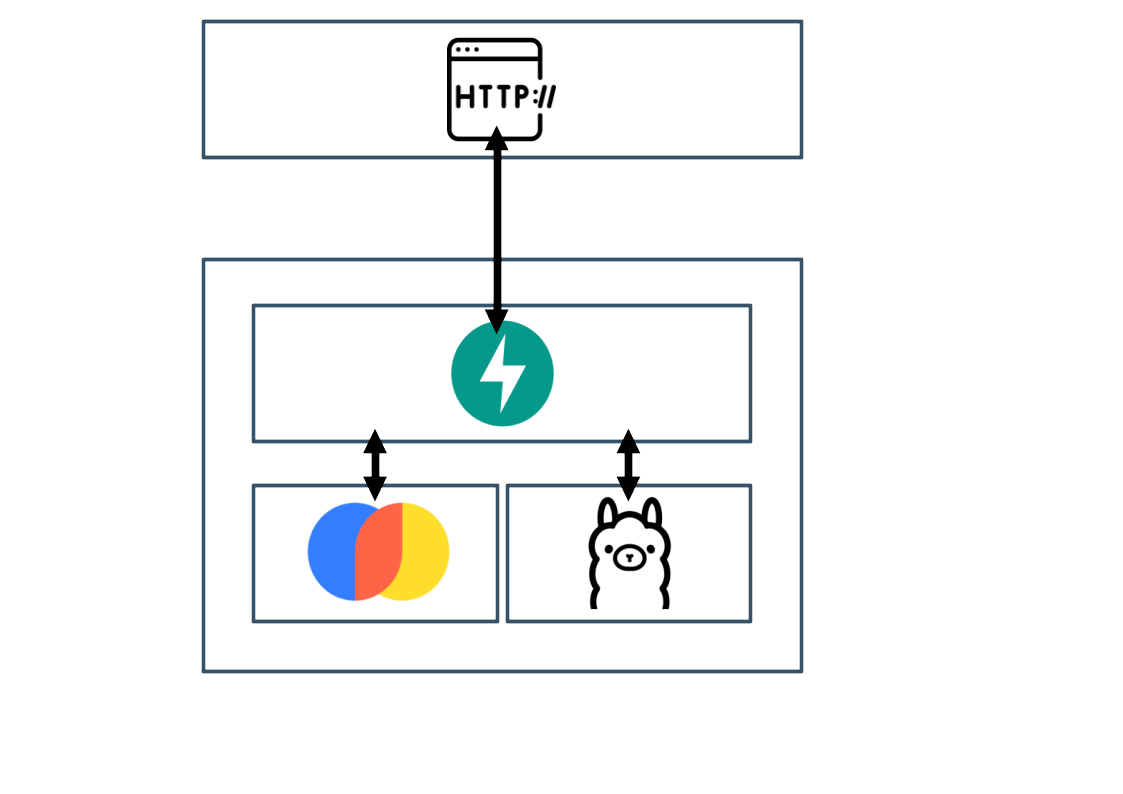
\includegraphics[width=1\linewidth]{Imagens/arquitetura.png}
    \caption{Arquitetura do Assistente de Buscas} 
    \label{fig:arq-assist-busca}
\end{figure}

% AFAZER: Alterar figura

\section{Banco Vetorial}
\label{sec:Assistente.1}
\subsection{Chroma DB}
\label{subsec:Assistente.1.1}

Conforme descrito pelos seus desenvolvedores e mantenedores \cite{Chroma:1}, o Chroma DB é um projeto concebido e mantido por uma equipe dedicada de especialistas da empresa Chroma, se tratando de um banco de dados vetorial de código aberto, cujo desenvolvimento tem foco na garantia de integração nativa com aplicações de inteligência artificial. A arquitetura do Chroma DB foi projetada para simplificar e agilizar o desenvolvimento de aplicações baseadas em \ac{LLM}s, fornecendo mecanismos que permitem a modularização de conjuntos de dados, informações e documentos, facilitando sua integração com \ac{LLM}s. O Chroma DB disponibiliza ferramentas robustas para o armazenamento e gerenciamento de documentos e seus metadados, assim como a criação e persistência de sua representação por \textit{embeddings}, possibilitando a realização de buscas de similaridade semântica sobre os dados de forma otimizada.

Entre os pontos fortes do Chroma DB estão a facilidade de implantação e utilização, assim como a priorização da produtividade dos desenvolvedores, sem comprometer a eficiência e a rapidez das operações por ele realizadas. O banco vetorial funciona como um serviço de servidor e vem acompanhado de SDKs de alta qualidade, escritos em Python e JavaScript/TypeScript, os quais fornecem todo o ferramental necessário a uma integração fluida em diversos tipos de projetos. Ademais, apresenta compatibilidade com ambientes de desenvolvimento interativos, como os populares notebooks Jupyter e IPython, promovendo uma experiência mais colaborativa e ágil para desenvolvedores e cientistas de dados.

O núcleo organizacional do Chroma DB são as coleções (\textit{collections}), sendo estruturas nas quais \textit{embeddings}, documentos e metadados relacionados são armazenados e por meio das quais são gerenciados. Sua utilização se dá de forma simples e direta, sendo necessário apenas lhe atribuir um nome e iniciar a inserção dos documentos, visto que o banco vetorial já se encarrega automaticamente da geração dos \textit{embeddings} e da indexação correspondente. Embora, por padrão, o banco já tenha definidas uma função de geração de \textit{embeddings} e uma métrica de similaridade padrão (o modelo \textit{all-MiniLM-L6-v2}, do \textit{Sentence Transformers}, e distância euclidiana, respectivamente), para cenários que exigem maior flexibilidade, a plataforma permite o fornecimento de uma função de geração de \textit{embeddings} personalizada, possibilitando a utilização de modelos específicos, que atendam às particularidades e características de comportamento desejadas. Analogamente, é possível configurar a medida de similaridade, de forma que ela utilize outras métricas, em vez da padrão, como, por exemplo, a distância do cosseno, reconhecidamente eficaz para medida de distância de vetores de \textit{embeddings}.

Uma vez processado, o documento, juntamente com seu  id, \textit{embeddings} e metadados são armazenados na coleção, sendo sua representação vetorial indexada para dar suporte à busca por similaridade de forma eficiente. O Chroma DB faz uso de estruturas otimizadas, como grafos do tipo HNSW (\textit{Hierarchical Navigable Small World}) ou algoritmos de \textit{approximate nearest neighbor} (ANN) para recuperação de documentos com \textit{embeddings} mais semelhantes de forma mais rápida e com bom desempenho.

As consultas em uma coleção são realizadas por meio de se informar listas de textos de entrada, a partir dos quais o banco de vetores retorna uma quantidade definida e ajustável de resultados semanticamente mais semelhantes aos termos informados. Os resultados da consulta incluem, além do conteúdo e metadados dos documentos retornados, o valor  da distância semântica entre cada um deles e o texto de entrada, permitindo uma análise com maior granularidade e a validação da relevância dos conteúdos. Essa capacidade de análise de similaridade de forma intuitiva permite posterior processamento intermediário dos resultados (como, por exemplo, a possibilidade de filtragem dos resultados e o estabelecimento de um limiar de exclusão de resultados com base em uma similaridade mínima desejada), oferecendo mais flexibilidade para o processo como um todo.

Quando da realização de uma consulta ao banco vetorial, em uma coleção específica, a mesma função de geração de \textit{embeddings} utilizada para gerar as representações vetoriais armazenadas é executada sobre o texto/documento fornecido como critério de busca, resultando, similarmente, em uma representação em formato de vetor de alta dimensionalidade. O Chroma DB, então, realiza a busca dentre os documentos vetorizados já armazenados por instâncias semanticamente mais semelhantes, utilizando a métrica de similaridade definida na criação da coleção, recuperando os documentos resultantes da busca.

\subsection{Modelo da função de \textit{embeddings}}
\label{subsec:Assistente.1.2}

Considerando a possibilidade oferecida pelo banco vetorial de se fornecer uma função de geração de \textit{embeddings} personalizada, sopesamos a utilização de diferentes modelos, levando em conta seu desempenho para fins de cálculo de similaridade -- levando em conta, especificamente, os resultados sobre a amostra de dados utilizada neste estudo. Dentre os modelos avaliados, a opção feita foi pelo INSTRUCTOR-XL. Trata-se de um modelo desenvolvido pela equipe de pesquisa de Processamento de Linguagem Natural (NLP) da Universidade de Hong Kong, incluindo a participação de pesquisadores de outras instituições, como \textit{University of Washington}, Meta AI e \textit{Allen Institute for AI}, publicado em 2023 \cite{Instructor:1}. O modelo selecionado pertence à série de modelos INSTRUCTOR, que são projetados para gerar \textit{embeddings} de texto de alta qualidade e se baseiam na arquitetura Transformer, assim como modelos de estado da arte, como \ac{BERT} e \c{GPT}.

No trabalho de  \citeonline{Instructor:2}, os seus publicadores o definem como \textit{“One Embedder [for] Any Task”} e como

\begin{citacao}
    an instruction-finetuned text embedding model that can generate text embeddings tailored to any task (e.g., classification, retrieval, clustering, text evaluation, etc.) and domains (e.g., science, finance, etc.) by simply providing the task instruction, without any finetuning. \footnote{Um modelo de geração de \textit{embeddings} textuais com \textit{fine-tuning} feito a partir de uma instrução, capaz de gerar \textit{embeddings} de texto otimizados para qualquer tarefa (tais como, classificação, recuperação, agrupamento, avaliação de texto, etc.) e quaisquer domínios (quais sejam ciência, finanças, etc.) simplesmente fornecendo a instrução da tarefa, sem necessidade de \textit{fine-tuning} tradicional. (Tradução nossa)}
\end{citacao}

Os INSTRUCTORs são, portanto, modelos de criação de \textit{embeddings} textuais de forma adaptativa, a partir da inclusão de instruções em linguagem natural, as quais atuam como direcionadores de ajuste fino, demonstrando bom desempenho em não somente “compreender” texto em um sentido mais aberto e genérico, sendo capaz de interpretá-lo com uma visão direcionada a aplicações e casos de uso particulares. Desta forma, as representações vetoriais geradas são otimizadas para tarefas específicas (como classificação, recuperação de informações, agrupamento, avaliação semântica, entre outras) e/ou domínios diferentes sem a necessidade de refinamento do modelo nos moldes tradicionais de \textit{finetuning}, tornando-o adaptável e mais relevante para diversas aplicações.
A versão utilizada no Assistente de Busca, especificamente, é a \textit{instructor-xl}, sendo a variante dentre a família de modelos INSTRUCTOR com maior tamanho, otimizada para desempenho e equilíbrio entre precisão e eficiência em aplicações de processamento de linguagem natural.

\section{Geração de Conteúdo}
\label{sec:Assistente.2}

\subsection{LLaMA}
\label{subsec:Assistente.2.1}
O modelo LLaMA (\textit{Large Language Model Meta AI}) ou simplesmente Llama, foi proposto em artigo de fevereiro de 2023 \cite{Llama:1}, havendo sido projetado para pesquisas avançadas em \ac{PLN}. Sua publicação se deu com a intenção da Meta AI, responsável pelo desenvolvimento do modelo, de disponibilizar acesso por parte da comunidade acadêmica e de desenvolvedores a um recurso de alta capacidade, permitindo-lhes explorar aplicações de \ac{IA} e experimentar inovações em grandes modelos de linguagem.

Baseado na arquitetura \textit{Transformers}, similar ao modelo \ac{GPT}, o Llama é otimizado para balancear desempenho e eficiência, estando apto a ser utilizado em tarefas como geração de texto, resumo de documentos, tradução automática, e resposta a perguntas. Tendo várias versões com tamanhos que variam de 7 bilhões (7B) a 65 bilhões (65B) de parâmetros, a  coleção de modelos permite a escolha de uma opção mais adequada, conforme a aplicação desejada e os recursos computacionais disponíveis.

A Meta AI, em sua introdução ao projeto, afirma que o Llama foi projetado como alternativa a outros \ac{LLM}s, como o GPT da OpenAI, com foco em ser mais eficiente em termos de recursos computacionais. Nesse contexto, o modelo é definido como
\begin{citacao}
    a state-of-the-art foundational large language model designed to help researchers advance their work in this subfield of AI. Smaller, more performant models such as LLaMA enable others in the research community who don’t have access to large amounts of infrastructure to study these models, further democratizing access in this important, fast-changing field. \cite{Llama:2} \footnote{um LLM de propósito geral, de última geração, projetado para ajudar pesquisadores a avançarem em seus trabalhos neste subcampo da IA. Modelos menores e mais eficientes, como o LLaMA, permitem que outros na comunidade de pesquisa que não têm acesso a grandes infraestruturas estudem esses modelos, democratizando ainda mais o acesso a este campo importante e em rápida evolução. (Tradução nossa)}
\end{citacao}


Um dos pontos fortes do Llama no contexto dos \ac{LLM}s é precisamente este fato de ele exigir um poder computacional consideravelmente reduzido e recursos mais modestos em comparação com outros modelos de referência à época de seu lançamento, sendo, pela natureza de seu treinamento -- baseado em dados não rotulados -- ideal para ser refinado para uma ampla gama de aplicações e tarefas.

O artigo de publicação do modelo aponta que o treinamento do Llama incluiu um número de \textit{tokens} na ordem de trilhões e utilizou exclusivamente conjuntos de dados publicamente disponíveis, sem contar com dados em bancos de dados proprietários ou de acesso restrito. Quando do lançamento da versão original, a versão do Llama com 13 bilhões de parâmetros ofereceu melhor desempenho que o GPT-3, que utiliza 175 bilhões de parâmetros; assim como o LLaMA65B se mostrou  competitivo com modelos maiores, como Chinchilla-70B e PaLM-540B (com 70 e 540 milhões de parâmetros, respectivamente).

Ao realizar o lançamento do Llama, em fevereiro de 2023, com o intuito de manter a integridade e evitar o potencial mau uso do modelo mediante uma publicação não supervisionada, a Meta AI optou por realizar a disponibilização sob uma licença de uso não-comercial, com foco em aplicações para fins de pesquisa, apenas. O acesso ao modelo, então, era garantido mediante análise caso a caso para acadêmicos, para organizações civis e governamentais, como também para laboratórios da indústria internacional, a qual se seguia à submissão de manifestação de interesse.

No início do semestre seguinte, a Meta disponibilizou mais uma versão do modelo, o Llama 2 \cite{Llama:3}. Nessa nova liberação, foi tornado disponível, sem custos para pesquisas e uso comercial, os pesos e o código de inicialização para a versão pré-treinada e direcionada à conversação. Aprimoramentos foram aplicados por meio do uso de técnicas que consideram \textit{feedback} humano, como \textit{Reinforcement Learning with Human Feedback} (RLHF), coleta de dados sobre preferência nas interações com humanos,  modelagem de recompensa e uma técnica simples para evitar degradação na qualidade no seguimento das instruções dadas ao modelo, chamada \textit{Ghost Attention} (GAtt). \cite{Llama:4}

No ano de 2024, em maio, julho e novembro, a Meta AI fez o lançamento de atualizações do Llama, com suas versões 3, 3.1 e 3.2, respectivamente. Cada uma das versões trouxe avanços significativos em relação às diversas iterações do Llama 2, em especial no número de parâmetros (405 bilhões). O \textit{paper} de lançamento do Llama 3 o descreve como:
\begin{citacao}
    a herd of language models that natively support multilinguality, coding, reasoning, and tool usage, [whose largest version] is a dense Transformer with 405B parameters and a context window of up to 128K tokens [delivering] comparable quality to leading language models such as GPT-4 on a plethora of tasks. \cite{Llama:5} \footnote{um conjunto de modelos de linguagem com suporte nativo a multi-idiomas, codificação, raciocínio e uso de ferramentas, [cuja maior versão] é um Transformer denso com 405 bilhões de parâmetros e uma janela de contexto de até 128 mil tokens, [oferecendo] qualidade comparável a modelos de linguagem de ponta, como o GPT-4, em uma ampla variedade de tarefas. (Tradução nossa)}
\end{citacao}


A versão mais recente até a escrita deste estudo, o Llama 3.2, se intitula como um conjunto de modelos customizáveis com inteligência artificial de ponta e revolucionária, dados os avanços que demonstrou. Além de manter uma versão anterior, Llama 3.1, com o tamanho pleno de 405 bilhões de parâmetros, foram disponibilizadas, com o Llama 3.2, versões mais leves, com 1 e 3 bilhões de parâmetros, as quais apresentam capacidade de geração de texto em múltiplos idiomas, otimizadas para serem leves e realizarem sumarização e reescrita de texto, execução de instruções e tarefas afins localmente, \textit{on-device}. As versões médias, com 11 e 90 bilhões de parâmetros, além das capacidades textuais, suportam usos de caso de compreensão de imagem. Dentre as possibilidades, são citadas

\begin{citacao}
    document-level understanding including charts and graphs, captioning of images, and visual grounding tasks such as directionally pinpointing objects in images based on natural language descriptions. \cite{Llama:6} \footnote{compreensão em nível de documento, incluindo gráficos e tabelas, descrição de imagens e tarefas de correspondência visual, como identificação direcional de objetos em imagens com base em descrições em linguagem natural. (Tradução nossa)}
\end{citacao}

Conforme declarado pela própria Meta AI, o foco do Llama 3.2 se dá sobre a disponibilização de versões mais leves, ao custo de uma quantidade menor de parâmetros (3 milhões, na versão dita padrão, em vez de 405 da versão 3.1). Apesar do tamanho reduzido, o desempenho é ainda muito promissor para diversas tarefas de processamento de linguagem natural.

\subsection{Ollama}
\label{subsec:Assistente.2.2}
O Ollama foi utilizado como ferramenta facilitadora, de forma a fazer uso do Llama3.1 como a etapa final do processo de recuperação da informação com base no texto informado pelo usuário. Trata-se de um \textit{framework} de código aberto e multiplataforma cujo desenvolvimento foi realizado por uma equipe da empresa Ollama Inc., baseado no llama.cpp -- uma biblioteca de alto desempenho escrita em C++ e otimizada para utilização de \ac{LLM}s.

Tal ferramenta foi projetada com fins específicos de simplificar a implementação e operação de \ac{LLM}s sem a necessidade de infraestrutura em nuvem; o que permitiu o acesso e gerenciamento de modelos diversos, tais qual o Llama 3.1 e outras arquiteturas avançadas em máquinas locais. Essa abordagem promove maior privacidade, ao evitar a necessidade de envio dedados a servidores de terceiros, além de reduzir os custos operacionais, eliminando as taxas associadas à inferência baseada em nuvem. \cite{Ollama:1}

A plataforma oferece suporte tanto para hardware de uso comum quanto para equipamentos de alto desempenho, provendo otimização do uso de GPUs durante a utilização de modelos de diferentes níveis de complexidade, incluindo aqueles com bilhões de parâmetros. A interação com o \ac{LLM} em si é mediada pelo Ollama, o qual fornece tanto uma interface de linha de comando -- a qual é executada na máquina em que a ferramenta está instalada -- quanto uma forma de interação programática, por meio de uma API REST, permitindo integração com aplicações de diversos tipos e usos.

Além disso, o Ollama dispõe de uma variedade de modelos que podem ser instalados de forma ágil e simplificada, permitindo acessá-los e utilizá-los de forma rápida e sem empecilhos, tanto para lhes fazer uso tal qual são disponibilizados, quanto para lhes aplicar ajustes específicos, buscando atender a domínios particulares.

